\documentclass[11pt,a4paper]{article}
\usepackage[utf8]{inputenc}
\usepackage[T1]{fontenc}
\usepackage{amsmath}
\usepackage{amsfonts}
\usepackage{amssymb}
\usepackage{graphicx}
\usepackage{xcolor}
\usepackage[left=1.50in, right=1.00in, top=1.00in, bottom=1.00in]{geometry}
\begin{document}
	\title{GCES IT club}
	\vspace{2 in}
	\author{A B, C D2021}
	\maketitle
	\newpage
	\listoffigures
	\newpage
	\tableofcontents
	\newpage
	\section{abc}
	hdjh
	\section{Introduction}
	Gandaki
	\subsection{title}
	jk
	\\
	as fig \ref{fig:complexitylatex} shows the complexity of document setting.
	
\begin{figure}[h]
	\centering
	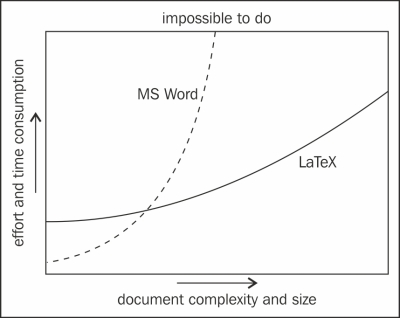
\includegraphics[width=0.5\linewidth]{Images/complexity_latex}
	\caption{Latex complexity}
	\label{fig:complexitylatex}
\end{figure}
	\subsubsection{title1}
	\textcolor{red} {math}
	\newpage
	\section{Math}
	$x=a+v$ is \textbf{formula} $\underline{\text{text}}$ \textit{to} \emph{text} eq \ref{eq:a}
	\begin{align}
	(a+b)^2 &= a^2 + 2\cdot \text{text} \times b +b^2 \nonumber\\ 
	a&= 5+b \nonumber\\
	n = [1,2,\cdots,6]
	\label{eq:a}
	\end{align}
	\section{List}
	\begin{itemize}
		\item hi
		\item hello
	\end{itemize}
	\begin{enumerate}
		\item hi
		\item hello
	\end{enumerate}
\section{table}
\begin{table}[h]
	\centering
	\caption{table}
	\label{tab:Table}
	\begin{tabular}{l|c|r}\hline
		SN&\multicolumn{2}{c}{Inputs} \\ \hline
		1& Hi & Hello \\ \hline
	\end{tabular}
\end{table}
\section{table}
\begin{table}[h]
	\centering
	\caption{table}
	\label{tab:Table}
	\begin{tabular}{l|c|r}\hline
		SN&\multicolumn{2}{c}{Inputs} \\ \hline
		1& Hi & Hello \\ \hline
	\end{tabular}
\end{table}
\end{document}